\documentclass[11pt,svgnames,smaller]{beamer}

\usepackage{CommandsAndStyle}

\usepackage{amsthm}
\usepackage{amsmath}
\usepackage{subfig}
\usepackage{xcolor}
\usepackage{textpos}
\usepackage{transparent}
\usepackage{tikz}
\usepackage{epigraph}
\usepackage[ruled,vlined,linesnumbered]{algorithm2e}
\usepackage{amsmath,amsfonts,amssymb,amsthm}
\usepackage{latexsym}
\usepackage{graphicx} % [demo] is just for the example
\usepackage{wrapfig}
\usepackage{array, makecell} %
\usepackage{hyperref}
\usepackage{soul}

\def\HiLiR{\leavevmode\rlap{\hbox to \hsize{\color{orange!30}\leaders\hrule height .8\baselineskip depth .5ex\hfill}}}
\def\HiLiG{\leavevmode\rlap{\hbox to \hsize{\color{green!30}\leaders\hrule height .8\baselineskip depth .5ex\hfill}}}
\def\HiLiB{\leavevmode\rlap{\hbox to \hsize{\color{blue!30}\leaders\hrule height .8\baselineskip depth .5ex\hfill}}}

\SetKwComment{Comment}{$\triangleright$\ }{}

\usepackage{caption}

\mode<presentation>

\author{Gaspare Ferraro}

\institute[University of Pisa]{University of Pisa\\Department of Computer Science}

\setbeamertemplate{section page}
{
	\begin{centering}
		\begin{beamercolorbox}[sep=16pt,center]{part title}
			\usebeamerfont{section title}\insertsection\par
		\end{beamercolorbox}
	\end{centering}
}

\title{TwoPaCo}
\subtitle{An efficient algorithm to build the compacted de Bruijn graph\\from many complete genomes}
\date{Pisa, 29 May 2018}
\titlegraphic{\vfill}
%\includegraphics[height=0.4cm]{images/creative_commons.png}}

\setbeamercolor{title}{fg=black!65!black}

\renewcommand{\partname}{Part}

\begin{document}
	
 \logo{\transparent{0.2}
\includegraphics[height=3cm]{images/cherubino}}

	\begin{frame} 
	\titlepage
	\end{frame}
			
	\part{Introduction}
\section{Introduction}

%%%%%%%%%%%%%%%%%%%%%%%%%%%%%%%%%%%%%%%%%%%%%%%%%%%%%%%%%%%%%%%%%%%%%%%%%%%%%%%%%%%%%%%%%%%%%%%%%%%%%%%%%%%%%%%%%%%%%%%%%%%
%%%%%%%%%%%%%%%%%%%%%%%%%%%%%%%%%%%%%%%%%%%%%%%%%%%%%%%%%%%%%%%%%%%%%%%%%%%%%%%%%%%%%%%%%%%%%%%%%%%%%%%%%%%%%%%%%%%%%%%%%%%

\begin{frame}
	\partpage
	\centering
\end{frame}

%%%%%%%%%%%%%%%%%%%%%%%%%%%%%%%%%%%%%%%%%%%%%%%%%%%%%%%%%%%%%%%%%%%%%%%%%%%%%%%%%%%%%%%%%%%%%%%%%%%%%%%%%%%%%%%%%%%%%%%%%%%
%%%%%%%%%%%%%%%%%%%%%%%%%%%%%%%%%%%%%%%%%%%%%%%%%%%%%%%%%%%%%%%%%%%%%%%%%%%%%%%%%%%%%%%%%%%%%%%%%%%%%%%%%%%%%%%%%%%%%%%%%%%

\begin{frame}
	\frametitle{A pan-genomic algorithm}
	\centering
	
	From the greek word \textit{pan} (everything)
	
	\medskip
	
	Given a series of complete genomes
	
	\medskip

	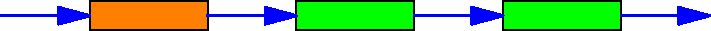
\includegraphics[height=0.4cm]{images/gen1}

  \medskip
  	
	
\includegraphics[height=0.4cm]{images/gen2}
	
	\medskip

  What we want to see:
  
  \begin{itemize}
    \item Similarities
    \item Differences
    \item Duplications
  \end{itemize}	
	
	\medskip
	
	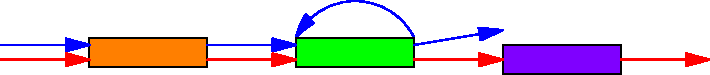
\includegraphics[height=1cm]{images/gen3}
	
\end{frame}

%%%%%%%%%%%%%%%%%%%%%%%%%%%%%%%%%%%%%%%%%%%%%%%%%%%%%%%%%%%%%%%%%%%%%%%%%%%%%%%%%%%%%%%%%%%%%%%%%%%%%%%%%%%%%%%%%%%%%%%%%%%
%%%%%%%%%%%%%%%%%%%%%%%%%%%%%%%%%%%%%%%%%%%%%%%%%%%%%%%%%%%%%%%%%%%%%%%%%%%%%%%%%%%%%%%%%%%%%%%%%%%%%%%%%%%%%%%%%%%%%%%%%%%

\begin{frame}
	\frametitle{de Bruijn graph}
	\centering
	  
  Sequence \#1: {\color{red} TGACGTC} ($2$-mers: {\color{red} TG GA AC CG GT TC})
  
  \medskip

	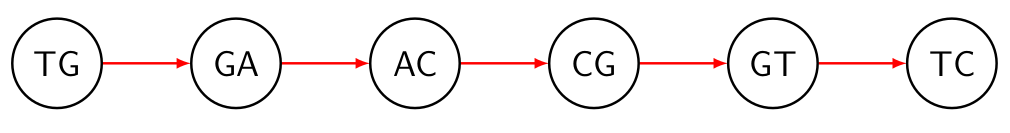
\includegraphics[height=0.7cm]{images/debruin-0}

  \medskip
  
  Sequence \#2: {\color{blue}TGACGTC} ($2$-mers: {\color{blue} TG GA AC CT TT TC})
	
	\medskip
	
	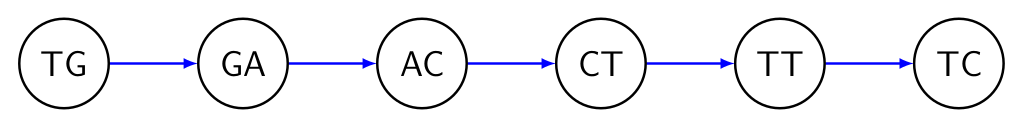
\includegraphics[height=0.7cm]{images/debruin-1}
	
	\medskip
	
	Find common vertices

	\medskip
  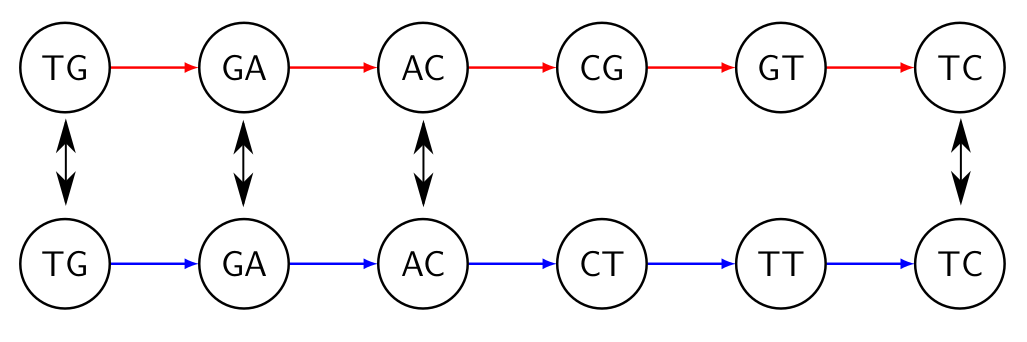
\includegraphics[height=1.5cm]{images/debruin-2}

  \medskip
  
  Merge them
	\medskip

	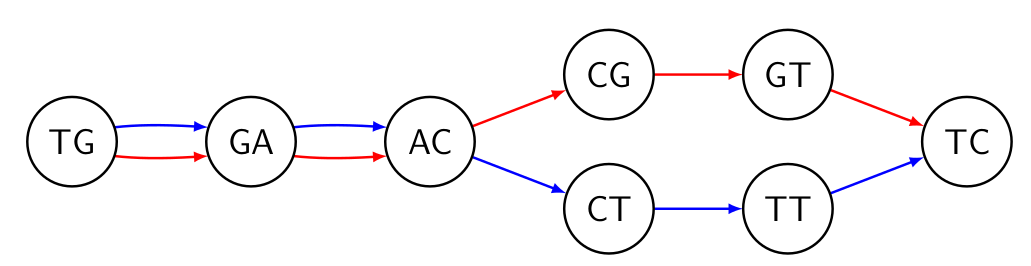
\includegraphics[height=1.3cm]{images/debruin-3}


\end{frame}

%%%%%%%%%%%%%%%%%%%%%%%%%%%%%%%%%%%%%%%%%%%%%%%%%%%%%%%%%%%%%%%%%%%%%%%%%%%%%%%%%%%%%%%%%%%%%%%%%%%%%%%%%%%%%%%%%%%%%%%%%%%
%%%%%%%%%%%%%%%%%%%%%%%%%%%%%%%%%%%%%%%%%%%%%%%%%%%%%%%%%%%%%%%%%%%%%%%%%%%%%%%%%%%%%%%%%%%%%%%%%%%%%%%%%%%%%%%%%%%%%%%%%%%

\begin{frame}
	\frametitle{Compacted de Bruijn graph}
	\centering
	
  To compact the de Bruijn graph we need to find the junctions
  
  \medskip
  
  A vertex is a junction if :
  
  Is the initial or final part of some sequence\\
  Has more than 1 in-edge or more than 1 out-edge\\
	
	\medskip

	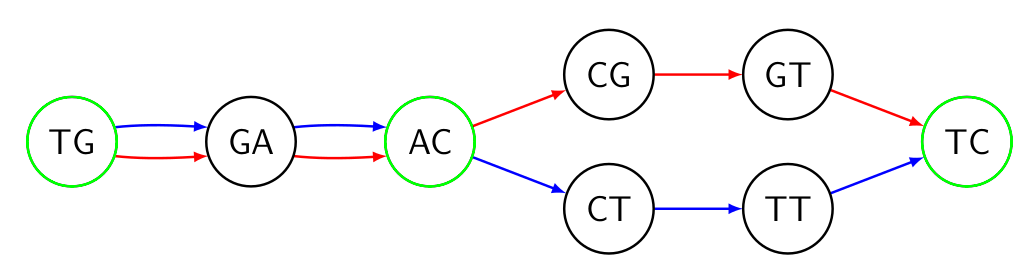
\includegraphics[height=2cm]{images/debruin-3a}

	\medskip

  Remove simple paths by connect junctions  	

	\medskip

	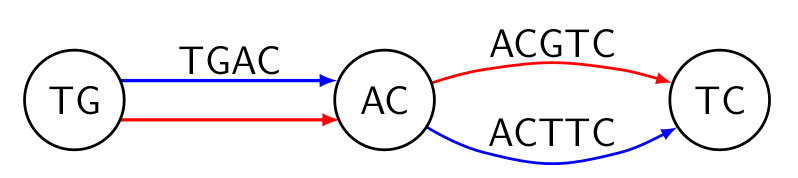
\includegraphics[height=1.5cm]{images/debruin-4}
	
\end{frame}

%%%%%%%%%%%%%%%%%%%%%%%%%%%%%%%%%%%%%%%%%%%%%%%%%%%%%%%%%%%%%%%%%%%%%%%%%%%%%%%%%%%%%%%%%%%%%%%%%%%%%%%%%%%%%%%%%%%%%%%%%%%
%%%%%%%%%%%%%%%%%%%%%%%%%%%%%%%%%%%%%%%%%%%%%%%%%%%%%%%%%%%%%%%%%%%%%%%%%%%%%%%%%%%%%%%%%%%%%%%%%%%%%%%%%%%%%%%%%%%%%%%%%%%

%\begin{frame}
%	\frametitle{Junctions}
%	\centering
%\end{frame}

%%%%%%%%%%%%%%%%%%%%%%%%%%%%%%%%%%%%%%%%%%%%%%%%%%%%%%%%%%%%%%%%%%%%%%%%%%%%%%%%%%%%%%%%%%%%%%%%%%%%%%%%%%%%%%%%%%%%%%%%%%%
%%%%%%%%%%%%%%%%%%%%%%%%%%%%%%%%%%%%%%%%%%%%%%%%%%%%%%%%%%%%%%%%%%%%%%%%%%%%%%%%%%%%%%%%%%%%%%%%%%%%%%%%%%%%%%%%%%%%%%%%%%%

\begin{frame}
	\frametitle{The problem}
	\centering
	
	How to construct the compacted de Bruijn graph,\\ from many complete genomes,\\ avoiding the ordinary graph construction?
	
	\medskip
	
	$\downarrow$
	
	\medskip

  
  \textbf{Which $k$-mers are junctions?}
  
  \medskip
  
  +
  
  \medskip
  
  How to construct the compacted de Bruijn graph given the junctions?
  
	
\end{frame}

	\part{The algorithm}
\section{The algorithm}

%%%%%%%%%%%%%%%%%%%%%%%%%%%%%%%%%%%%%%%%%%%%%%%%%%%%%%%%%%%%%%%%%%%%%%%%%%%%%%%%%%%%%%%%%%%%%%%%%%%%%%%%%%%%%%%%%%%%%%%%%%%
%%%%%%%%%%%%%%%%%%%%%%%%%%%%%%%%%%%%%%%%%%%%%%%%%%%%%%%%%%%%%%%%%%%%%%%%%%%%%%%%%%%%%%%%%%%%%%%%%%%%%%%%%%%%%%%%%%%%%%%%%%%

\begin{frame}
	\partpage
	\centering
\end{frame}

%%%%%%%%%%%%%%%%%%%%%%%%%%%%%%%%%%%%%%%%%%%%%%%%%%%%%%%%%%%%%%%%%%%%%%%%%%%%%%%%%%%%%%%%%%%%%%%%%%%%%%%%%%%%%%%%%%%%%%%%%%%
%%%%%%%%%%%%%%%%%%%%%%%%%%%%%%%%%%%%%%%%%%%%%%%%%%%%%%%%%%%%%%%%%%%%%%%%%%%%%%%%%%%%%%%%%%%%%%%%%%%%%%%%%%%%%%%%%%%%%%%%%%%

\begin{frame}
	\frametitle{Naive algorithm}
	\centering
	
	
	\begin{itemize}
	  \item[\textcolor{orange}{\textbullet}] Store all $(k+1)$-mers in a hash table
	  \item[\textcolor{green}{\textbullet}] For each $k$-mers query the possible edges
	  \item[\textcolor{blue}{\textbullet}] If only 1 in and 1 out edge, unmark as a junction
	\end{itemize}
	   
	%\medskip
	
   \scalebox{.55}{                        
   \begin{algorithm}[H]
      \small
       \DontPrintSemicolon
       \SetKwInOut{Input}{Input}
       \SetKwInOut{Output}{Output}
       \Input{$S = \{s_{1}, ..., s_{m}\}$ genoma sequences\\$k$ integer, size of $k$-mers\\ $E$ empty set data structure\\$C$ Candidate set of junctions (\textbf{naively all positions are marked})}
       \Output{A reduce candidate set of junctions $C$}
       
       \BlankLine
       \ForEach{$s \in S$}{
       \For{$1 \leq i < |s| - k $}{
        \If{$C[s,i] = marked$}{ 
        \HiLiR $E \gets E \cup  s[i..i+k] \cup  s[i-1..i+k-1]$ \Comment*[r]{Store all $(k+1)$-mers}
          }
        }
       }
       \BlankLine
       \ForEach{$s \in S$}{
        \For{$1 \leq i < |s| - k $}{
          \If{$C[s,i] = marked$}{
          
            $(in, out) \gets (0, 0)$ \Comment*[r]{Count in/out edges}
            
            \HiLiG\ForEach{$c \in \{A, C, G, T\}$}{
              \HiLiG \If{$v \cdot c \in E$}{
              \HiLiG$in \gets in + 1$\;
              }
              \HiLiG \If{$c \cdot v \in E$}{
              \HiLiG$out \gets out + 1$\;
              }
            }
            
            \HiLiB \If{$(in, out) = (1,1)$}{
            \HiLiB $C[s,i] = unmarked$ \Comment*[r]{surely not a junction}
            }
          }
        }
       }
              
       \Return{$C$}
       \caption{\textsc{Filter-Junctions}}
   \end{algorithm}
   }
   
\end{frame}

%%%%%%%%%%%%%%%%%%%%%%%%%%%%%%%%%%%%%%%%%%%%%%%%%%%%%%%%%%%%%%%%%%%%%%%%%%%%%%%%%%%%%%%%%%%%%%%%%%%%%%%%%%%%%%%%%%%%%%%%%%%
%%%%%%%%%%%%%%%%%%%%%%%%%%%%%%%%%%%%%%%%%%%%%%%%%%%%%%%%%%%%%%%%%%%%%%%%%%%%%%%%%%%%%%%%%%%%%%%%%%%%%%%%%%%%%%%%%%%%%%%%%%%

\begin{frame}
	\frametitle{The memory issue}
	
	  First part of the naive algorithm:
	  
	  \bigskip
	  
	  \ForEach{$s \in S$}{
      \For{$1 \leq i < |s| - k $}{
          \If{$C[s,i] = marked$}{
            $E \gets E \cup  s[i..i+k] \cup  s[i-1..i+k-1]$\;
        }
      }
    }
     
	 \centering

  \pause
  
    \bigskip

    We don't really need and, in almost all pratical cases, \\ we can't store all the possible $(k+1)$-mers.
    
    \bigskip
    
    Mainly because \textbf{only a little percentual} of them are \\ junction in the de Bruijn graph.
      
\end{frame}

%%%%%%%%%%%%%%%%%%%%%%%%%%%%%%%%%%%%%%%%%%%%%%%%%%%%%%%%%%%%%%%%%%%%%%%%%%%%%%%%%%%%%%%%%%%%%%%%%%%%%%%%%%%%%%%%%%%%%%%%%%%
%%%%%%%%%%%%%%%%%%%%%%%%%%%%%%%%%%%%%%%%%%%%%%%%%%%%%%%%%%%%%%%%%%%%%%%%%%%%%%%%%%%%%%%%%%%%%%%%%%%%%%%%%%%%%%%%%%%%%%%%%%%

\begin{frame}
	\frametitle{Bloom filter}
	
	\centering

	A space-efficient probabilistic hash table
	
	\medskip
	
	Bitmap $V$ of size $b$, $h$ hash functions $f_{0}, f_{1}, ..., f_{h-1} : U \rightarrow [0, b-1]$ \\
		
	\medskip
	
	insertion($x$) $\rightarrow V[f_{i}(x)] = 1$, $\forall$ $0 \leq i < h$ 
	
	\medskip
	
	contains($x$) $\rightarrow$ \textbf{probabily yes} if $V[f_{i}(x)] == 1$, $\forall$ $0 \leq i < h$
  \medskip
  
  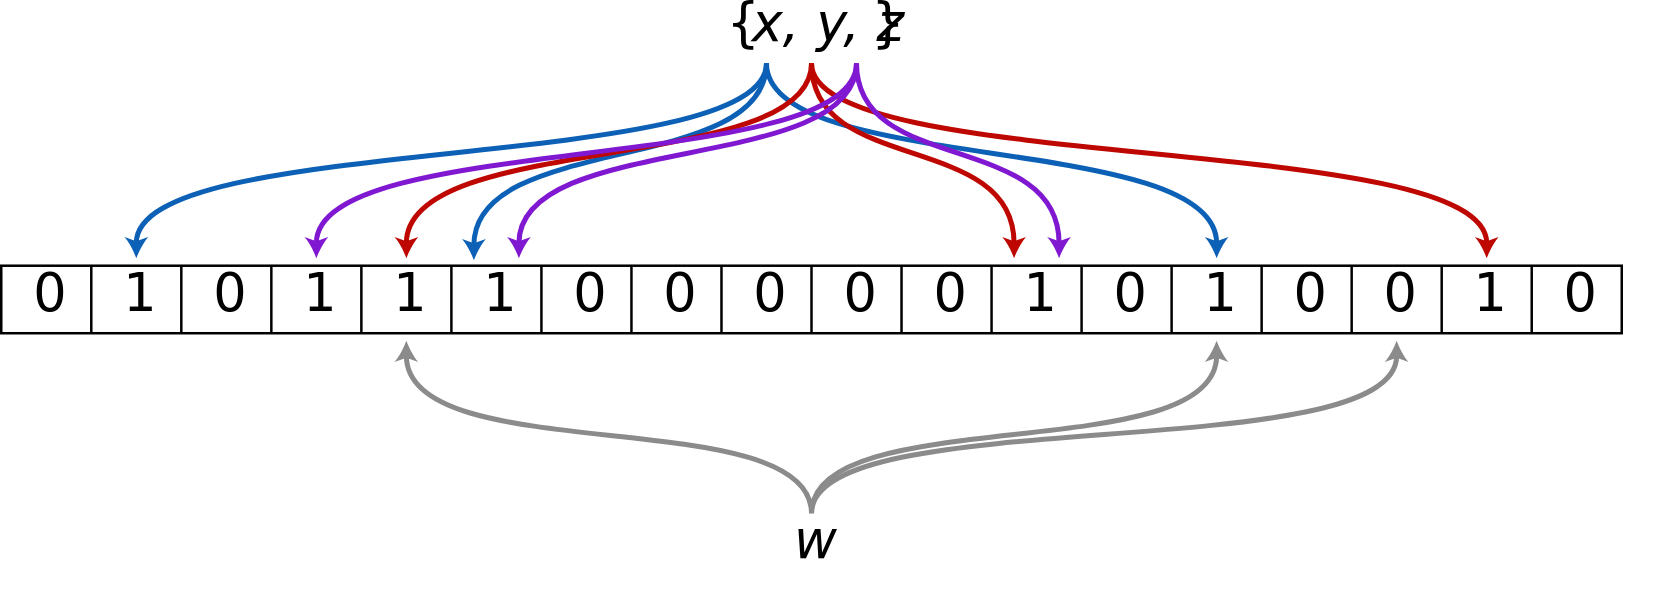
\includegraphics[height=3cm]{images/bloom_filter}
  
  \medskip
	Probability of false positive, after $n$ insertion: $p_{FP} \simeq (1 - e^{-hn/m})^{h}$
	
	
\end{frame}

%%%%%%%%%%%%%%%%%%%%%%%%%%%%%%%%%%%%%%%%%%%%%%%%%%%%%%%%%%%%%%%%%%%%%%%%%%%%%%%%%%%%%%%%%%%%%%%%%%%%%%%%%%%%%%%%%%%%%%%%%%%
%%%%%%%%%%%%%%%%%%%%%%%%%%%%%%%%%%%%%%%%%%%%%%%%%%%%%%%%%%%%%%%%%%%%%%%%%%%%%%%%%%%%%%%%%%%%%%%%%%%%%%%%%%%%%%%%%%%%%%%%%%%

\begin{frame}
	\frametitle{Two Pass version}
	\centering
	
	\begin{itemize}
	  \item[\textcolor{orange}{\textbullet}] First pass: Select a set of junction candidates by insert all the $(k+1)$-mers in a bloom filter of choosing size
	  \item[\textcolor{green}{\textbullet}] Second pass: Filter out the false positive by storing the reduce sets of $(k+1)$-mers in an hash table
	\end{itemize}

   \scalebox{.8}{                        
   \begin{algorithm}[H]
      \small
       \DontPrintSemicolon
       \SetKwInOut{Input}{Input}
       \SetKwInOut{Output}{Output}
       \Input{strings $S = \{s_{1}, ..., s_{m}\}$ genoma sequences\\integer $k$, size of $k$-mers\\integer $b$, size of bloom filter\\ Candidate set of junctions $C_{in}$ (\textbf{naively all positions are marked})}
       \Output{A reduce candidate set of junctions $C_{out}$}
       
       \BlankLine
       
       \HiLiR$F \gets$ empty bloom filter of size $b$ \Comment*[r]{First pass}
       \HiLiR$C_{temp} \gets \textsc{Filter-Junctions}(S, k, F, C_{in})$  \;

       \BlankLine

       \HiLiG$H \gets$ empty hash table \Comment*[r]{Second pass}
       \HiLiG$C_{out} \gets \textsc{Filter-Junctions}(S, k, H, C_{in})$ \;

       \BlankLine
              
       \Return{$C_{out}$}
       \caption{\textsc{Filter-Junctions-Two-Pass}}
   \end{algorithm}
   }
   

\end{frame}

%%%%%%%%%%%%%%%%%%%%%%%%%%%%%%%%%%%%%%%%%%%%%%%%%%%%%%%%%%%%%%%%%%%%%%%%%%%%%%%%%%%%%%%%%%%%%%%%%%%%%%%%%%%%%%%%%%%%%%%%%%%
%%%%%%%%%%%%%%%%%%%%%%%%%%%%%%%%%%%%%%%%%%%%%%%%%%%%%%%%%%%%%%%%%%%%%%%%%%%%%%%%%%%%%%%%%%%%%%%%%%%%%%%%%%%%%%%%%%%%%%%%%%%

\begin{frame}
	\frametitle{The memory issue$^{2}$}
	\centering
	
	How much memory do we use now?
	
	\medskip
	
	\begin{itemize}
	  \item First pass: Bloom filter of size $b$ (of our decision)
	  \item Second pass: Hash table containing $(k+1)$-mers of junction candidates
	\end{itemize}

	\medskip
	
	We don't know the possible size of the hash table in the second pass. \\
	What if the hash table is not small enough?
  
  \pause 
  
	\medskip

  \textbf{Solution}: Split the input $k$-mers in chunks and analyze them in multiple rounds.

  \medskip
  
  Split \textit{TGACTACTGAC} in $3$ chunks of $3$-mers: \\
  
  \medskip
  
  \st{
  Wrong: \{
    {\color{red}TGA} 
    {\color{blue}GAC}
    {\color{pink}ACT}
  \}, 
  \{
    {\color{green}CTA} 
    {\color{darkgreen}TAC}
    {\color{pink}ACT}
  \}, 
  \{
    {\color{orange}CTG} 
    {\color{red}TGA} 
    {\color{blue}GAC}
  \}
  }
  
  \medskip
  
  Correct: \{
    {\color{red}TGA} 
    {\color{red}TGA} 
    {\color{orange}CTG} 
  \}, 
  \{
    {\color{blue}GAC}
    {\color{blue}GAC}
    {\color{green}CTA} 
  \}, 
  \{
    {\color{pink}ACT}
    {\color{pink}ACT}
    {\color{darkgreen}TAC} 
  \}  
\end{frame}

%%%%%%%%%%%%%%%%%%%%%%%%%%%%%%%%%%%%%%%%%%%%%%%%%%%%%%%%%%%%%%%%%%%%%%%%%%%%%%%%%%%%%%%%%%%%%%%%%%%%%%%%%%%%%%%%%%%%%%%%%%%
%%%%%%%%%%%%%%%%%%%%%%%%%%%%%%%%%%%%%%%%%%%%%%%%%%%%%%%%%%%%%%%%%%%%%%%%%%%%%%%%%%%%%%%%%%%%%%%%%%%%%%%%%%%%%%%%%%%%%%%%%%%

\begin{frame}
	\frametitle{$k$-mers splitting}
	\centering
	
	\begin{itemize}
	  \item[\textcolor{orange}{\textbullet}] Count how many $k$-mers are mapped in each of the $c$ hash value ($c = 2^{l}$)
	  \item[\textcolor{green}{\textbullet}] Iterate over all the hash value and insert them in the current chunk
	  \item[\textcolor{blue}{\textbullet}] If the size of current chunks exceeds the average pass to the next chunk
	\end{itemize}

		\scalebox{0.65}{                        
   \begin{algorithm}[H]
      \small
       \DontPrintSemicolon
       \SetKwInOut{Input}{Input}
       \SetKwInOut{Output}{Output}
       \Input{strings $S = \{s_{1}, ..., s_{m}\}$ genoma sequences\\integer $k$, size of $k$-mers\\integer $b$, size of bloom filter\\integer $l$, number of rounds\\function $f(x)$, from $k$-mers to integers}
       \Output{$(V_{0}, V_{1}, \ldots, V_{l-1} )$ chunks of $k$-mers}
       
       \BlankLine
       
       $V_{0} \gets \emptyset, V_{1} \gets \emptyset, \ldots, V_{l-1} \gets \emptyset$ \Comment*[r]{Chunks, initially empty}
       $c_{0} \gets 0, c_{1} \gets 0, \ldots, c_{q-1} \gets 0$ \Comment*[r]{Counters, for balancing $k$-mers}
       %$F \gets$ empty Bloom filter of size $b$\;
       
        \BlankLine
        
       \HiLiR$c_{i} \gets | \{$ $k$-mer $x \mid f(x) = i$ \} $|$ \;

	     % \ForEach{$s \in S$}{
       %   \For{$1 \leq i < |s| - k $}{
       %       \If{$s[i..i+k-1]$ not in $F$}{
       %       Insert $s[i..i+k-1]$ in $F$ \;
       %       $c_{f(s[i..i+k-1])} \gets c_{f(s[i..i+k-1])} + 1$ \;
       %     }
       %   }
       % }
        
       \HiLiR$T \gets \sum_{0 \leq t < q} c_{t}/l $  \Comment*[r]{Average size of a chunk}
        
       \BlankLine
       
       $idx \gets 0$ \;
       \For{$0 \leq i < q $}{
         \HiLiG$V_{idx} = V_{idx} \cup \{i\}$ \Comment*[r]{Add $i$ to the current chunk}
         \HiLiB\If{$|V_{idx}| \geq T$}{
          \HiLiB$idx \gets \min(idx+1, l-1)$ \Comment*[r]{Next chunk, until reach $l-1$}
         }
       }

       \BlankLine
              
       \Return{$(V_{0}, V_{1}, \ldots, V_{l-1} )$}
       \caption{\textsc{Round-Splitting}}
    \end{algorithm}
    
    }
\end{frame}
	
	
%%%%%%%%%%%%%%%%%%%%%%%%%%%%%%%%%%%%%%%%%%%%%%%%%%%%%%%%%%%%%%%%%%%%%%%%%%%%%%%%%%%%%%%%%%%%%%%%%%%%%%%%%%%%%%%%%%%%%%%%%%%
%%%%%%%%%%%%%%%%%%%%%%%%%%%%%%%%%%%%%%%%%%%%%%%%%%%%%%%%%%%%%%%%%%%%%%%%%%%%%%%%%%%%%%%%%%%%%%%%%%%%%%%%%%%%%%%%%%%%%%%%%%%

\begin{frame}

	\frametitle{Multiple rounds: dealing with memory restrictions}
	\centering
		
	\begin{itemize}
	  \item[\textcolor{orange}{\textbullet}] Partitionate the input with \textsc{Round-Splitting}
	  \item[\textcolor{green}{\textbullet}] Analyse each partition with \textsc{Filter-Junctions-Two-Pass}
	  \item[\textcolor{blue}{\textbullet}] Merge the results of each rounds and output the real junctions
	\end{itemize}
	
	\medskip
	
	\scalebox{0.75}{                        
   \begin{algorithm}[H]
      \small
       \DontPrintSemicolon
       \SetKwInOut{Input}{Input}
       \SetKwInOut{Output}{Output}
       \Input{strings $S = \{s_{1}, ..., s_{m}\}$ genoma sequences\\integer $k$, size of $k$-mers\\integer $b$, size of bloom filter\\integer $l$, number of rounds\\function $f(x)$, from $k$-mers to integers }
       \Output{$C_{final}$ all the junctions in the compacted de Bruijn graph}
       
       \BlankLine
       
       \HiLiR$(V_{0}, V_{1}, \ldots, V_{l-1} ) \gets \textsc{Round-Splitting}$($S$, $k$, $b$, $l$, $f$) \Comment*[r]{Create chunks}
       $C_{init} \gets$ Boolean array with every position unmarked \;

       \BlankLine
       
       \HiLiG\For{$0 \leq i < l$\Comment*[r]{For each chunks}}
       {
       \HiLiG  $C_{i} \gets$ mark every position of $C_{init}$ that starts a $k$-mer with hash in $V_{i}$ \;
       \HiLiG$C_{i} \gets$ \textsc{Filter-Junctions-Two-Pass}($S$, $k$, $b$, $C_{i}$) \Comment*[r]{Find junctions}
       }

       \BlankLine
  
       \HiLiB$C_{final} = \bigcup{C_{i}}$ \Comment*[r]{Merge junctions of each chunks}
       
       \BlankLine
              
       \Return{$C_{final}$}
       \caption{\textsc{TwoPaCo}}
   \end{algorithm}
   }
   


\end{frame}

%%%%%%%%%%%%%%%%%%%%%%%%%%%%%%%%%%%%%%%%%%%%%%%%%%%%%%%%%%%%%%%%%%%%%%%%%%%%%%%%%%%%%%%%%%%%%%%%%%%%%%%%%%%%%%%%%%%%%%%%%%%
%%%%%%%%%%%%%%%%%%%%%%%%%%%%%%%%%%%%%%%%%%%%%%%%%%%%%%%%%%%%%%%%%%%%%%%%%%%%%%%%%%%%%%%%%%%%%%%%%%%%%%%%%%%%%%%%%%%%%%%%%%%

\begin{frame}
	\frametitle{Parallelization scheme}
	\centering
	
	As far we focused in reducing memory. What about the time?
	
	\pause
	
	\bigskip
	
	TwoPaCo can be easily parallelizable:
	
	\begin{itemize}
	  \item Parallel for loops (OpenMP, TBB, ...)
	  \item Concurrent bloom filter (parallel insert and search)
	  \item Concurrent hash table (parallel insert and search)
	\end{itemize}
	
	\pause
	
	\medskip
	
	We made a clever usage of the concurrent data structs:
	
	\begin{itemize}
	  \item Only insertion in the first part
	  \item Only query in the second part (static table, no race conditions)
	\end{itemize}
	
	
	
\end{frame}

	\part{Results}

\begin{frame}
	\partpage
	\centering
\end{frame}

	
	\section{Conclusion}
	
	\begin{frame}
  \frametitle{References}
  
  [1] Minkin, I., Pham, S., Medvedev, P. (2016). 
  
  \textbf{TwoPaCo}: An efficient algorithm to build the compacted de Bruijn graph from many complete genomes	  

  \medskip
  
  [2] Minkin, I., Patel, A., Kolmogorov, M., Vyahhi, N., Pham, S. (2013). 
  
  \textbf{Sibelia}: a scalable and comprehensive synteny block generation tool for closely related microbial
genomes.

  \medskip
  
  [3] Marcus, S., Lee, H., Schatz, M. C. (2014). 
  
  \textbf{SplitMEM}: a graphical algorithm for pan-genome analysis with suffix skips.

  \medskip

  [4] Baier, U., Beller, T., Ohlebusch, E. (2015). 
  
  Graphical pan-genome analysis with compressed suffix trees and the \textbf{Burrows-Wheeler transform}.

	\end{frame}

	\begin{frame}
		\frametitle{Questions}
		\centering
		\Large
		Thanks for your attention!
		
		\bigskip
		
		Questions?
 	\end{frame}
 	
 	
 	%%%%%%%%%%%%%%%%%%%%%%%%%%%%%%%%%%%%%%%%%%
 	
 		\begin{frame}
		\frametitle{My results}
		\centering
		
    Source code:
    
    {\color{blue}https://github.com/GaspareG/TwoPaCo/blob/master/srcgas/twopaco.cpp}
		
		\bigskip
		
			\begin{tabular}{ | r | r | r | r | r | r | r | }
      \hline
        Dataset &  k & Version & Time &    Initial & First Pass & Second Pass \\ \hline
        
       2 E.coli & 25 & BF+HT   &  {\color{green}18s}  & 10.207.478 &    392.836 &     177.396 \\ 
       2 E.coli & 25 & BF      &    {\color{red}29s}  & 10.207.478 &          - &     177.396 \\ \hline
       
       4 E.coli & 25 & BF+HT   &  {\color{green}38s}  & 20.301.208 &  1.261.345 &     676.686 \\ 
       4 E.coli & 25 & BF      &    {\color{red}64s}  & 20.301.208 &          - &     676.686 \\ \hline
       
       8 E.coli & 25 & BF+HT   &  {\color{green}87s}  & 39.871.914 &  3.231.119 &   1.822.718 \\ 
       8 E.coli & 25 & BF      &   {\color{red}134s}  & 39.871.914 &          - &   1.822.718 \\ \hline
       
      16 E.coli & 25 & BF+HT   & {\color{green}160s}  & 77.848.026 &  7.076.460 &   4.046.561 \\ 
      16 E.coli & 25 & BF      &   {\color{red}280s}  & 77.848.026 &          - &   4.046.561 \\ 
      \hline
      \end{tabular}

      \medskip
      
  		Running time and junctions candidate after each pass
  		
 	\end{frame}
  
\end{document}
